\documentclass[11pt]{article}

\usepackage[margin=1in]{geometry}
\usepackage{setspace}
\onehalfspacing
\usepackage{graphicx}
\graphicspath{report_images/}
\usepackage{appendix}
\usepackage{listings}
\usepackage{float}
\usepackage{amsthm}
% The next three lines make the table and figure numbers also include section number
\usepackage{chngcntr}
\counterwithin{table}{section}
\counterwithin{figure}{section}
% Needed to make titling page without a page number
\usepackage{titling}

% DOCUMENT INFORMATION =================================================
\title {ECEN 429: Introduction to Digital Systems Design Laboratory \\ North Carolina Agricultural and Technical State University \\ Department of Electrical and Computer Engineering} % Declare Title
\author{Reporter: Chris Cannon\\ \and Partner: Nikiyah Beulah} % Declare authors
\date{February 8, 2018}
% ======================================================================

\begin{document}

\begin{titlingpage}
\maketitle
\begin{center}
	Lab 3
\end{center}
\end{titlingpage}

\section{Introduction}
This lab focuses on building increasingly complex systems that build on each other, which will give us more experience with integrating systems using components. Code reuse is important for any type of software development, including VHDL. Therefore, it is important that we understand how to nest components to build more complex systems from basic building blocks. We start by creating an adder circuit for two 2-bit numbers, and we build more complex circuits that utilize those systems for more advanced operations.

\section{Background, Design Solution, and Results}

\subsection{Problem 1 Bit Slicer}

\subsubsection{Background}
For this problem, we are to create a bit slicer that will add two 2-bit numbers 'a' and 'b', as well has handling a carry-in bit 'cin'.

\theoremstyle{definition}
\newtheorem{definition}{Definition}
\begin{definition}
Carry-in Bit: the carry-in bit represents a 1-bit overflow from a previous addition operation. Because a full adder is intended to be modular, and build adders of multiple bits, it is important that the previous operation be available. For purposes of this lab, the carry-in for a 1 bit adder will be tied to ground.
\end{definition}

The concept of a 2-bit adder was covered in Lab 2, so we had a good starting point for this lab. For reference, the truth table for a single 2-bit adder is defined in ~\ref{tab:fullAddTruthTable}.

\begin{table}[h]
\begin{center}
	\begin{tabular}{| l | l | l | l | l |}
		\hline
		A & B & CI & SUM & CO \\ \hline
		0 & 0 & 0 & 0 & 0 \\ \hline
		0 & 0 & 1 & 1 & 0 \\ \hline
		0 & 1 & 0 & 1 & 0 \\ \hline
		0 & 1 & 1 & 0 & 1 \\ \hline
		1 & 0 & 0 & 1 & 0 \\ \hline
		1 & 0 & 1 & 0 & 1 \\ \hline
		1 & 1 & 0 & 0 & 1 \\ \hline
		1 & 1 & 1 & 1 & 1 \\ \hline
	\end{tabular}
	\caption{\label{tab:fullAddTruthTable}Truth table for a full adder.}
	\label{tab:fullAddTruthTable}
\end{center}
\end{table}

\subsubsection{Design Solution}
To implement our design, we decided to use two full-adders. We were able to reuse our code from Lab 2 to create the full-adder entity, and then implement this design using two components. Because we abstracted our full-adder using a component, we had to write less actual code, which made our solution both cleaner and easier to read. For our inputs, we used 'a2' and 'a1' to represent our first 2-bit number, and 'b2' and 'b1' to represent our second 2-bit number. 'ci' of course represents out carry-in bit. The output sum is represented by bits `x2` and `x1`, and the carry-out bit is represented as `cout`. The truth table for this entire circuit is given in Table ~\ref{tab:stupidlyLongSlicerTruthTable}. The pin assignments for this design are given in Table ~\ref{tab:slicerPinAssignments}.

\begin{definition}
	Carry-out Bit: the carry-out bit represents a 1-bit overflow from the current addition operation. This can either be used to signal an error condition or to tie this adder in with multiple full adders. The result of this addition operation will either between 0 and 3. If the output is 2 or 3, the carry-out bit will be HIGH to signal that there is an additional bit needed to represent the results of this operation.
\end{definition}

\begin{table}[H]
\begin{center}
	\begin{tabular}{| l | l | l | l | l | l | l | l |}
		\hline
		cin & a2 & a1 & b2 & b1 & cout & x2 & x1 \\ \hline
		0 & 0 & 0 & 0 & 0 & 0 & 0 & 0 \\ \hline
		0 & 0 & 0 & 0 & 1 & 0 & 0 & 1 \\ \hline
		0 & 0 & 0 & 1 & 0 & 0 & 1 & 0 \\ \hline
		0 & 0 & 0 & 1 & 1 & 0 & 1 & 1 \\ \hline
		0 & 0 & 1 & 0 & 0 & 0 & 0 & 1 \\ \hline
		0 & 0 & 1 & 0 & 1 & 0 & 1 & 0 \\ \hline
		0 & 0 & 1 & 1 & 0 & 0 & 1 & 1 \\ \hline
		0 & 0 & 1 & 1 & 1 & 1 & 0 & 0 \\ \hline
		0 & 1 & 0 & 0 & 0 & 0 & 1 & 0 \\ \hline
		0 & 1 & 0 & 0 & 1 & 0 & 1 & 1 \\ \hline
		0 & 1 & 0 & 1 & 0 & 1 & 0 & 0 \\ \hline
		0 & 1 & 0 & 1 & 1 & 1 & 0 & 1 \\ \hline
		0 & 1 & 1 & 0 & 0 & 0 & 1 & 1 \\ \hline
		0 & 1 & 1 & 0 & 1 & 1 & 0 & 0 \\ \hline
		0 & 1 & 1 & 1 & 0 & 1 & 0 & 1 \\ \hline
		0 & 1 & 1 & 1 & 1 & 1 & 1 & 0 \\ \hline
		1 & 0 & 0 & 0 & 0 & 0 & 0 & 1 \\ \hline
		1 & 0 & 0 & 0 & 1 & 0 & 1 & 0 \\ \hline
		1 & 0 & 0 & 1 & 0 & 0 & 1 & 1 \\ \hline
		1 & 0 & 0 & 1 & 1 & 1 & 0 & 0 \\ \hline
		1 & 0 & 1 & 0 & 0 & 0 & 1 & 0 \\ \hline
		1 & 0 & 1 & 0 & 1 & 0 & 1 & 1 \\ \hline
		1 & 0 & 1 & 1 & 0 & 1 & 0 & 0 \\ \hline
		1 & 0 & 1 & 1 & 1 & 1 & 0 & 1 \\ \hline
		1 & 1 & 0 & 0 & 0 & 0 & 1 & 1 \\ \hline
		1 & 1 & 0 & 0 & 1 & 1 & 0 & 0 \\ \hline
		1 & 1 & 0 & 1 & 0 & 1 & 0 & 1 \\ \hline
		1 & 1 & 0 & 1 & 1 & 1 & 1 & 0 \\ \hline
		1 & 1 & 1 & 0 & 0 & 1 & 0 & 0 \\ \hline
		1 & 1 & 1 & 0 & 1 & 1 & 0 & 1 \\ \hline
		1 & 1 & 1 & 1 & 0 & 1 & 1 & 0 \\ \hline
		1 & 1 & 1 & 1 & 1 & 1 & 1 & 1 \\ \hline
	\end{tabular}
	\caption{\label{tab:stupidlyLongSlicerTruthTable}Truth table for the problem 1 solution.}
\end{center}
\end{table}

\begin{table}[H]
\begin{center}
	\begin{tabular}{| l | l | l |}
		\hline
		Bit & Label & Port \\ \hline
		a1 & Switch 0 & V17 \\ \hline
		a2 & Switch 1 & V16 \\ \hline
		b1 & Switch 2 & W16 \\ \hline
		b2 & Switch 3 & W17 \\ \hline
		cin & Switch 4 & W15 \\ \hline
		x1 & LED 0 & U16 \\ \hline
		x2 & LED 1 & E19 \\ \hline
		cout & LED 2 & V19 \\ \hline
	\end{tabular}
	\caption{\label{tab:slicerPinAssignments}Port assignment for each bit used in Problem 1.}
\end{center}
\end{table}

\subsubsection{Results}
A select number of input and output combinations are shown in Figures ~\ref{fig:SlicerAllOff} through ~\ref{fig:SlicerOnePlusTwoPlusTwo}.

\begin{figure}[H]
\begin{center}
	\includegraphics[width=0.3\textwidth]{./report-images/Part1/IMG_3032.jpg}
	\caption{\label{fig:SlicerAllOff}In this state, all inputs are off, therefore, there is no output. We know this because LED 0, LED 1, and LED 2 are all off. The decimal equivalent is 0 + 0 + 0 = 0.}
\end{center}
\end{figure}

\begin{figure}[H]
\begin{center}
	\includegraphics[width=0.3\textwidth]{./report-images/Part1/IMG_3033.jpg}
	\caption{\label{fig:SlicerZeroPlusOne}In this state, there is no carry-in because Switch 4 is off, B is 00 because Switches 2 and 3 are off, A is 01 because Switch 0 is on and Switch 1 is off. This results in a sum of 01 with no carry, so only LED 0 is on. The decimal equivalent is 0 + 0 + 1 = 1.}
\end{center}
\end{figure}

\begin{figure}[H]
\begin{center}
	\includegraphics[width=0.3\textwidth]{./report-images/Part1/IMG_3034.jpg}
	\caption{\label{fig:SlicerOnePlusOne}In this state, there is no carry-in because Switch 4 is off, B is 01 because Switch 3 is off and Switch 2 is on, A is 01 because Switch 0 is on and Switch 1 is off. This results in a sum of 10 with no carry, so only LED 1 is on. The decimal equivalent is 0 + 1 + 1 = 2.}
\end{center}
\end{figure}

\begin{figure}[H]
\begin{center}
	\includegraphics[width=0.3\textwidth]{./report-images/Part1/IMG_3035.jpg}
	\caption{\label{fig:SlicerOnePlusOnePlusOne}In this state, there is a carry-in because Switch 4 is on, B is 01 because Switch 3 is off and Switch 2 is on, A is 01 because Switch 0 is on and Switch 1 is off. This results in a sum of 11 with no carry, so only LED 0 is on. The decimal equivalent is 1 + 1 + 1 = 3.}
\end{center}
\end{figure}

\begin{figure}[H]
\begin{center}
	\includegraphics[width=0.3\textwidth]{./report-images/Part1/IMG_3036.jpg}
	\caption{\label{fig:SlicerOnePlusTwoPlusTwo}In this state, there is a carry-in because Switch 4 is on, B is 11 because Switches 2 and 3 on, A is 11 because Switches 0 and 1 are on. This results in a sum of 11 with a carry-out, so all output LEDs 0, 1, and 2 are on. The decimal equivalent is 1 + 3 + 3 = 7.}
\end{center}
\end{figure}


\subsection{Problem 2 2:1 Multiplexer}

\subsubsection{Background}
Using the bit slicer developed in Problem 1, we will feed the outputs into a 2:1 multiplexer with a 1-bit `sel` input. 

\begin{definition}
	Multiplexer: A multiplexer, or mux, is a digital device that can "pass-through" values depending on a selector input. For example, a 2:1 mux with a 1-bit selector and inputs 'a' and 'b' will output input 'a' when the selector input is '0' or LOW and will output 'b' when the selector input is '1' or HIGH.
\end{definition}

The multiplexer in this problem is supposed to output the sum of the bit slicer operation when the 'sel' bit is '1' or HIGH. The sum refers to \textit{only} the two bit output of the sum operation. In this lab, we referred to these outputs as 'x2' and 'x1', where 'x2' is the most significant bit. When the 'sel' bit is '0' or LOW, the circuit is supposed to output the carry-out bit 'cout'. 

\subsubsection{Design Solution}
To implement this design, we reused the code from Problem one, and used it as a component. Therefore, we only had to declare and instantiate the component, not redefine the architecture. Based on the assignment given in the Background section above, we knew that we had to basically double our truth table. If the 'sel' bit is HIGH or '1', we will output 'x2' and 'x1'. When the 'sel' bit is LOW or '0', we will output just the 'cout' bit. Tables ~\ref{tab:selOneTruthTable} and ~\ref{tab:selZeroTruthTable} provide the truth tables for this design. We have summarized our port assignments in Table ~\ref{tab:ledMuxPorts}.

\begin{table}[H]
\begin{center}
	\begin{tabular}{| l | l | l |}
		\hline
		Bit & Label & Port \\ \hline
		a1 & Switch 0 & V17 \\ \hline
		a2 & Switch 1 & V16 \\ \hline
		b1 & Switch 2 & W16 \\ \hline
		b2 & Switch 3 & W17 \\ \hline
		cin & Switch 4 & W15 \\ \hline
		sel & Switch 5 & V15 \\ \hline
		x1 & LED 0 & U16 \\ \hline
		x2 & LED 1 & E19 \\ \hline
		cout & LED 2 & V19 \\ \hline
	\end{tabular}
	\caption{\label{tab:ledMuxPorts}Input and output pin assignments for the multiplexer circuit.}
\end{center}	
\end{table}


\begin{table}[H]
\begin{center}
	\begin{tabular}{| l | l | l | l | l | l | l | l | l |}
		\hline
		sel & cin & a2 & a1 & b2 & b1 & cout & x2 & x1 \\ \hline
		1 & 0 & 0 & 0 & 0 & 0 & 0 & 0 & 0 \\ \hline
		1 & 0 & 0 & 0 & 0 & 1 & 0 & 0 & 1 \\ \hline
		1 & 0 & 0 & 0 & 1 & 0 & 0 & 1 & 0 \\ \hline
		1 & 0 & 0 & 0 & 1 & 1 & 0 & 1 & 1 \\ \hline
		1 & 0 & 0 & 1 & 0 & 0 & 0 & 0 & 1 \\ \hline
		1 & 0 & 0 & 1 & 0 & 1 & 0 & 1 & 0 \\ \hline
		1 & 0 & 0 & 1 & 1 & 0 & 0 & 1 & 1 \\ \hline
		1 & 0 & 0 & 1 & 1 & 1 & 0 & 0 & 0 \\ \hline
		1 & 0 & 1 & 0 & 0 & 0 & 0 & 1 & 0 \\ \hline
		1 & 0 & 1 & 0 & 0 & 1 & 0 & 1 & 1 \\ \hline
		1 & 0 & 1 & 0 & 1 & 0 & 0 & 0 & 0 \\ \hline
		1 & 0 & 1 & 0 & 1 & 1 & 0 & 0 & 1 \\ \hline
		1 & 0 & 1 & 1 & 0 & 0 & 0 & 1 & 1 \\ \hline
		1 & 0 & 1 & 1 & 0 & 1 & 0 & 0 & 0 \\ \hline
		1 & 0 & 1 & 1 & 1 & 0 & 0 & 0 & 1 \\ \hline
		1 & 0 & 1 & 1 & 1 & 1 & 0 & 1 & 0 \\ \hline
		1 & 1 & 0 & 0 & 0 & 0 & 0 & 0 & 1 \\ \hline
		1 & 1 & 0 & 0 & 0 & 1 & 0 & 1 & 0 \\ \hline
		1 & 1 & 0 & 0 & 1 & 0 & 0 & 1 & 1 \\ \hline
		1 & 1 & 0 & 0 & 1 & 1 & 0 & 0 & 0 \\ \hline
		1 & 1 & 0 & 1 & 0 & 0 & 0 & 1 & 0 \\ \hline
		1 & 1 & 0 & 1 & 0 & 1 & 0 & 1 & 1 \\ \hline
		1 & 1 & 0 & 1 & 1 & 0 & 0 & 0 & 0 \\ \hline
		1 & 1 & 0 & 1 & 1 & 1 & 0 & 0 & 1 \\ \hline
		1 & 1 & 1 & 0 & 0 & 0 & 0 & 1 & 1 \\ \hline
		1 & 1 & 1 & 0 & 0 & 1 & 0 & 0 & 0 \\ \hline
		1 & 1 & 1 & 0 & 1 & 0 & 0 & 0 & 1 \\ \hline
		1 & 1 & 1 & 0 & 1 & 1 & 0 & 1 & 0 \\ \hline
		1 & 1 & 1 & 1 & 0 & 0 & 0 & 0 & 0 \\ \hline
		1 & 1 & 1 & 1 & 0 & 1 & 0 & 0 & 1 \\ \hline
		1 & 1 & 1 & 1 & 1 & 0 & 0 & 1 & 0 \\ \hline
		1 & 1 & 1 & 1 & 1 & 1 & 0 & 1 & 1 \\ \hline
	\end{tabular}
	\caption{\label{tab:selOneTruthTable}This table shows the outputs displayed when the 'sel' bit is '1' or HIGH. The only output should be from the sum bits 'x2' and 'x1'.}
\end{center}	
\end{table}

\begin{table}[H]
\begin{center}
	\begin{tabular}{| l | l | l | l | l | l | l | l | l |}
		\hline
		sel & cin & a2 & a1 & b2 & b1 & cout & x2 & x1 \\ \hline
		0 & 0 & 0 & 0 & 0 & 0 & 0 & 0 & 0 \\ \hline
		0 & 0 & 0 & 0 & 0 & 1 & 0 & 0 & 0 \\ \hline
		0 & 0 & 0 & 0 & 1 & 0 & 0 & 0 & 0 \\ \hline
		0 & 0 & 0 & 0 & 1 & 1 & 0 & 0 & 0 \\ \hline
		0 & 0 & 0 & 1 & 0 & 0 & 0 & 0 & 0 \\ \hline
		0 & 0 & 0 & 1 & 0 & 1 & 0 & 0 & 0 \\ \hline
		0 & 0 & 0 & 1 & 1 & 0 & 0 & 0 & 0 \\ \hline
		0 & 0 & 0 & 1 & 1 & 1 & 1 & 0 & 0 \\ \hline
		0 & 0 & 1 & 0 & 0 & 0 & 0 & 0 & 0 \\ \hline
		0 & 0 & 1 & 0 & 0 & 1 & 0 & 0 & 0 \\ \hline
		0 & 0 & 1 & 0 & 1 & 0 & 1 & 0 & 0 \\ \hline
		0 & 0 & 1 & 0 & 1 & 1 & 1 & 0 & 0 \\ \hline
		0 & 0 & 1 & 1 & 0 & 0 & 0 & 0 & 0 \\ \hline
		0 & 0 & 1 & 1 & 0 & 1 & 1 & 0 & 0 \\ \hline
		0 & 0 & 1 & 1 & 1 & 0 & 1 & 0 & 0 \\ \hline
		0 & 0 & 1 & 1 & 1 & 1 & 1 & 0 & 0 \\ \hline
		0 & 1 & 0 & 0 & 0 & 0 & 0 & 0 & 0 \\ \hline
		0 & 1 & 0 & 0 & 0 & 1 & 0 & 0 & 0 \\ \hline
		0 & 1 & 0 & 0 & 1 & 0 & 0 & 0 & 0 \\ \hline
		0 & 1 & 0 & 0 & 1 & 1 & 1 & 0 & 0 \\ \hline
		0 & 1 & 0 & 1 & 0 & 0 & 0 & 0 & 0 \\ \hline
		0 & 1 & 0 & 1 & 0 & 1 & 0 & 0 & 0 \\ \hline
		0 & 1 & 0 & 1 & 1 & 0 & 1 & 0 & 0 \\ \hline
		0 & 1 & 0 & 1 & 1 & 1 & 1 & 0 & 0 \\ \hline
		0 & 1 & 1 & 0 & 0 & 0 & 0 & 0 & 0 \\ \hline
		0 & 1 & 1 & 0 & 0 & 1 & 1 & 0 & 0 \\ \hline
		0 & 1 & 1 & 0 & 1 & 0 & 1 & 0 & 0 \\ \hline
		0 & 1 & 1 & 0 & 1 & 1 & 1 & 0 & 0 \\ \hline
		0 & 1 & 1 & 1 & 0 & 0 & 1 & 0 & 0 \\ \hline
		0 & 1 & 1 & 1 & 0 & 1 & 1 & 0 & 0 \\ \hline
		0 & 1 & 1 & 1 & 1 & 0 & 1 & 0 & 0 \\ \hline
		0 & 1 & 1 & 1 & 1 & 1 & 1 & 0 & 0 \\ \hline
	\end{tabular}
	\caption{\label{tab:selZeroTruthTable}This table shows the outputs displayed when the 'sel' bit is '0' or LOW. The only output should be the carry-out bit 'cout'.}
\end{center}
\end{table}

\subsubsection{Results}
A selected number of input/output combinations are displayed in Figures ~\ref{fig:BitMuxAllOff} through FIXHERE.

\begin{figure}[H]
\begin{center}
	\includegraphics[width=0.4\textwidth]{./report-images/Part2/IMG_0468.jpg}
	\caption{\label{fig:BitMuxAllOff}In this state, there is no carry in because Switch 4 is off, and the numbers being summed are all 0 because Switches 0 through 3 are off. Therefore, the 2 output LEDs 0 and 1 are off. The select input, Switch 5, is irrelevant to this operation.}
\end{center}
\end{figure}

\begin{figure}[H]
\begin{center}
	\includegraphics[width=0.4\textwidth]{./report-images/Part2/IMG_0469.jpg}
	\caption{\label{fig:BitMuxOnePlusOneCarry}In this state, there is no carry in because Switch 4 is off, B is 01 because Switch 3 is off and Switch 2 is on. A is 01 because Switch 0 is on and Switch 1 is off. Therefore, the decimal sum is 1+1 = 2. The select input, Switch 5, is i0 which means the carry-out bit should be displayed. Since there is no carry-out in this operation, LEDs 0 and 1 are off.}
\end{center}
\end{figure}

\begin{figure}[H]
\begin{center}
	\includegraphics[width=0.4\textwidth]{./report-images/Part2/IMG_0470.jpg}
	\caption{\label{fig:BitMuxOnePlusOneSum}In this state, there is no carry in because Switch 4 is off, sum should be displayed because Switch 5 is on. B is 01 because Switch 3 is off and Switch 2 is on. A is 01 because Switch 1 is off and Switch 0 is on. The decimal equivalent of this operation is 0+1+1 = 2. Because sum is to be displayed, LED 1 is on and LED 0 is off.}
\end{center}
\end{figure}

\begin{figure}[H]
\begin{center}
	\includegraphics[width=0.4\textwidth]{./report-images/Part2/IMG_0471.jpg}
	\caption{\label{fig:BitMuxOnePlusOnePlusOneSum}In this state, there is a carry in because Switch 4 is on, sum should be displayed because Switch 5 is on. B is 01 because Switch 3 is off and Switch 2 is on. A is 01 because Switch 1 is off and Switch 0 is on. The decimal equivalent of this operation is 1+1+1 = 3. Because sum is to be displayed, LEDs 1 and 0 are on.}
\end{center}
\end{figure}

\begin{figure}[H]
\begin{center}
	\includegraphics[width=0.4\textwidth]{./report-images/Part2/IMG_0472.jpg}
	\caption{\label{fig:BitMuxOnePlusOnePlusOneOverFlow}In this state, there is a carry in because Switch 4 is on, carry-out should be displayed because Switch 5 is off. B is 01 because Switch 3 is off and Switch 2 is on. A is 01 because Switch 1 is off and Switch 0 is on. The decimal equivalent of this operation is 1+1+1 = 3. Because carry-out is to be displayed, LEDs 1 and 0 are off because 3 can be represented in 2 bits.}
\end{center}
\end{figure}
	
\begin{figure}[H]
\begin{center}
	\includegraphics[width=0.4\textwidth]{./report-images/Part2/IMG_0473.jpg}
	\caption{\label{fig:BitMuxOnePlusTwoPlusOneOverFlow}In this state, there is no carry in because Switch 4 is off, carry-out should be displayed because Switch 5 is off. B is 10 because Switch 2 is off and Switch 3 is on. A is 01 because Switch 1 is off and Switch 0 is on. The decimal equivalent of this operation is 0+2+1 = 3. Because carry-out is to be displayed, and 2 can be represented in 2-bits so there is no carry-out, all LEDs are off.}
\end{center}
\end{figure}

\begin{figure}[H]
\begin{center}
	\includegraphics[width=0.4\textwidth]{./report-images/Part2/IMG_0474.jpg}
	\caption{\label{fig:BitMuxZeroPlusTwoPlusOneSum}In this state, there is no carry in because Switch 4 is off, sumshould be displayed because Switch 5 is on. B is 10 because Switch 2 is off and Switch 3 is on. A is 01 because Switch 1 is off and Switch 0 is on. The decimal equivalent of this operation is 0+2+1 = 3. Because sum is to be displayed, LEDs 1 and 0 are both on.}
\end{center}
\end{figure}

\begin{figure}[H]
\begin{center}
	\includegraphics[width=0.4\textwidth]{./report-images/Part2/IMG_0475.jpg}
	\caption{\label{fig:BitMuxAllOn}In this state, there is a carry in because Switch 4 is on, sum should be displayed because Switch 5 is on. B is 11 because Switches 2 and 3 are on. A is 11 because Switches 0 and 1 are on. The decimal equivalent of this operation is 1+3+3 = 7. Because sum is to be displayed, only the amount of the sum that can be represented in 2 bits will be shown. Therefore, LED 0 and LED 1 are both on.}
\end{center}
\end{figure}

\subsection{Problem 3 2:1 Multiplexer with Seven-Segment Output}

\subsubsection{Background}
For this problem, we are to utilize the seven-segment display to output our result from the circuit in Problem 2. Basically, if we are to output the sum, then we should display 0, 1, 2, or 3 on the seven-segment display. If we are to display the carry-out, then we will display 0 or 1.

\subsubsection{Design Solution}
The truth table for this circuit will be the same truth table shown in Figures ~\ref{tab:selZeroTruthTable} and ~\ref{tab:selOneTruthTable}, however output will be shown utilizing the seven-segment displays. A diagram of a segment display is shown in Figure ~\ref{fig:sevenSegFigure}.

\begin{figure}[h]
\begin{center}
	\includegraphics[width=0.2\textwidth]{../Lab2/report-images/img1.png}
	\caption{\label{fig:sevenSegFigure}Diagram of seven-segment display showing the assigned letter for each segment.}
\end{center}
\end{figure}

The basic flow of the system is a case statement including a series of if statements. We first determined  the input of the multiplexer to see if the circuit should display the sum or the carry-out bit. Once we decided which to display, the series of if statements will calculate what the proper output will be. The port assignments for Problem 3 are summarized in Table ~\ref{tab:sevSegPortMap}.

\begin{table}[H]
\begin{center}
	\begin{tabular}{| l | l | l |}
		\hline
		Bit & Label & Port \\ \hline
		a1 & Switch 0 & V17 \\ \hline
		a2 & Switch 1 & V16 \\ \hline
		b1 & Switch 2 & W16 \\ \hline
		b2 & Switch 3 & W17 \\ \hline
		cin & Switch 4 & W15 \\ \hline
		sel & Switch 5 & V15 \\ \hline
		out1 & Seven Seg A & W7 \\ \hline
		out2 & Seven Seg B & W6 \\ \hline
		out3 & Seven Seg C & U8 \\ \hline
		out4 & Seven Seg D & V8 \\ \hline
		out5 & Seven Seg E & U5 \\ \hline
		out6 & Seven Seg F & V5 \\ \hline
		out7 & Seven Seg G & U7 \\ \hline
	\end{tabular}
	\caption{\label{tab:sevSegPortMap}Port assignments for Problem 3.}
\end{center}
\end{table}

\subsubsection{Results}
This portion was totally successful and a selection of results are shown in Figures ~\ref{fig:sevSegAllOff} through ~\ref{fig:sevSegOnePlusOneSUM}.

\begin{figure}[H]
\begin{center}
	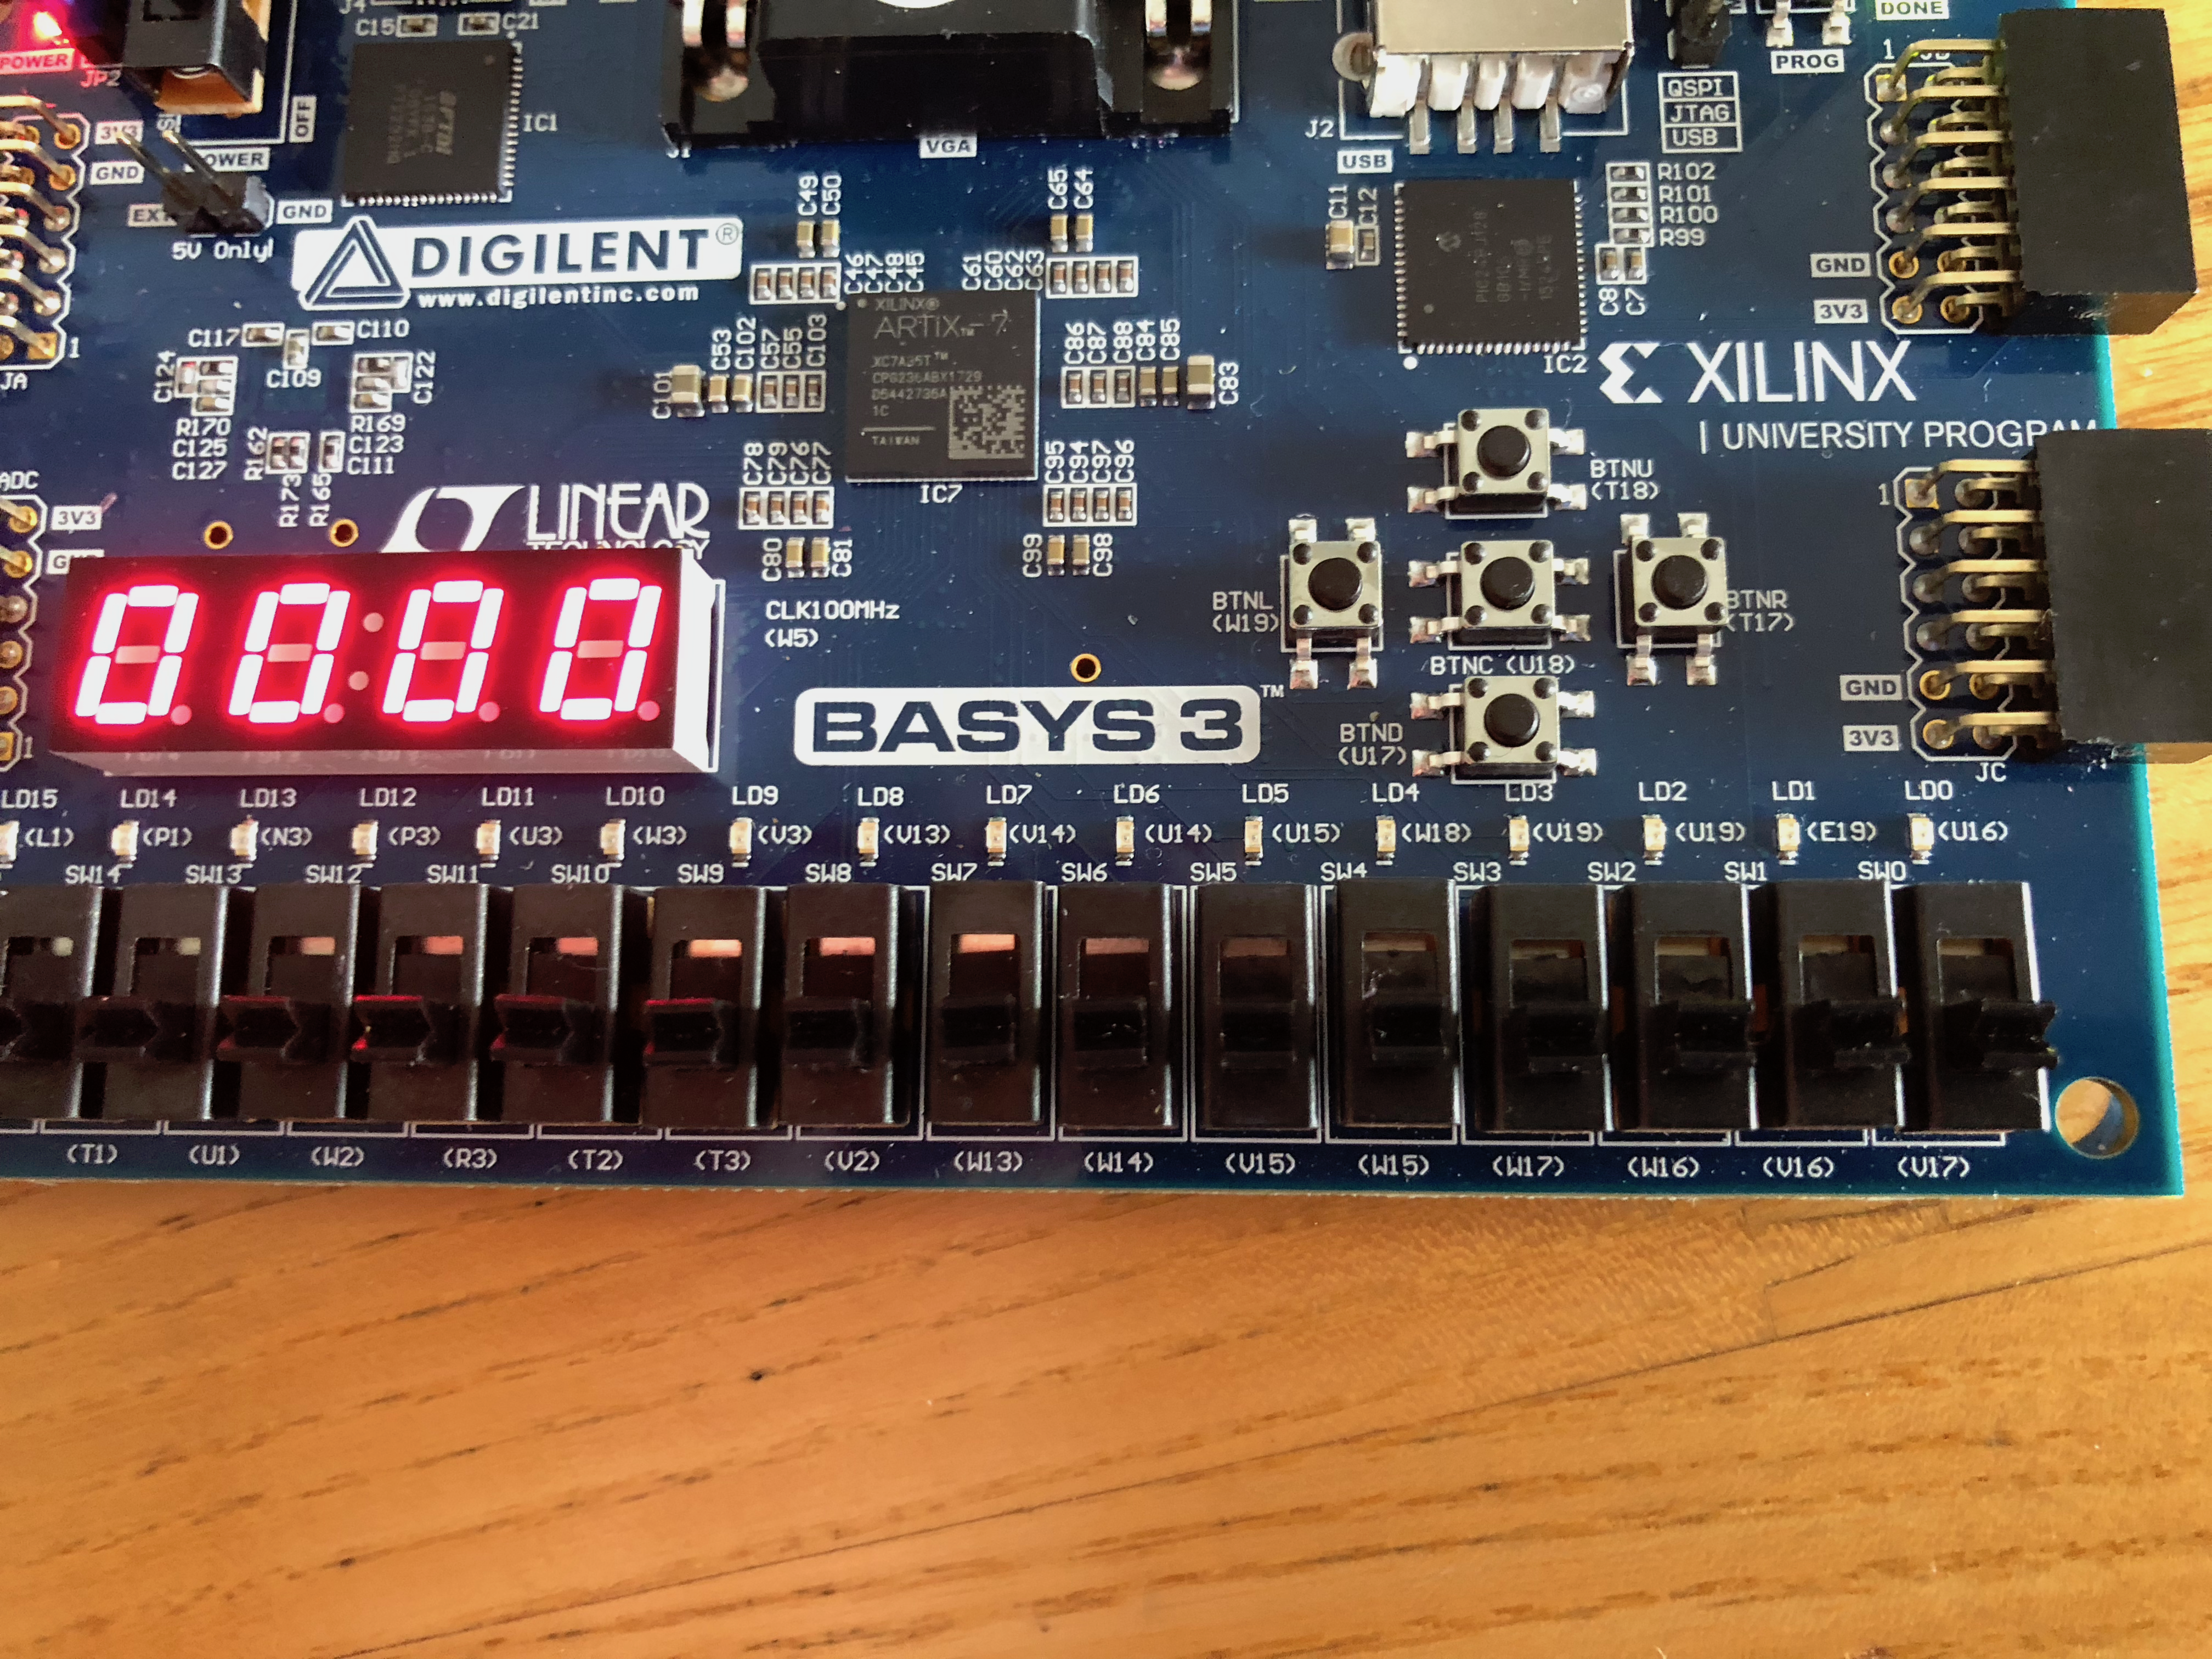
\includegraphics[width=0.4\textwidth]{./report-images/Part3/IMG_0476.png}
	\caption{\label{fig:sevSegAllOff}In this image, both the sum and the carry out are zero, because all input switches are off. Therefore, the seven-segment display reads 0.}
\end{center}
\end{figure}

\begin{figure}[H]
\begin{center}
	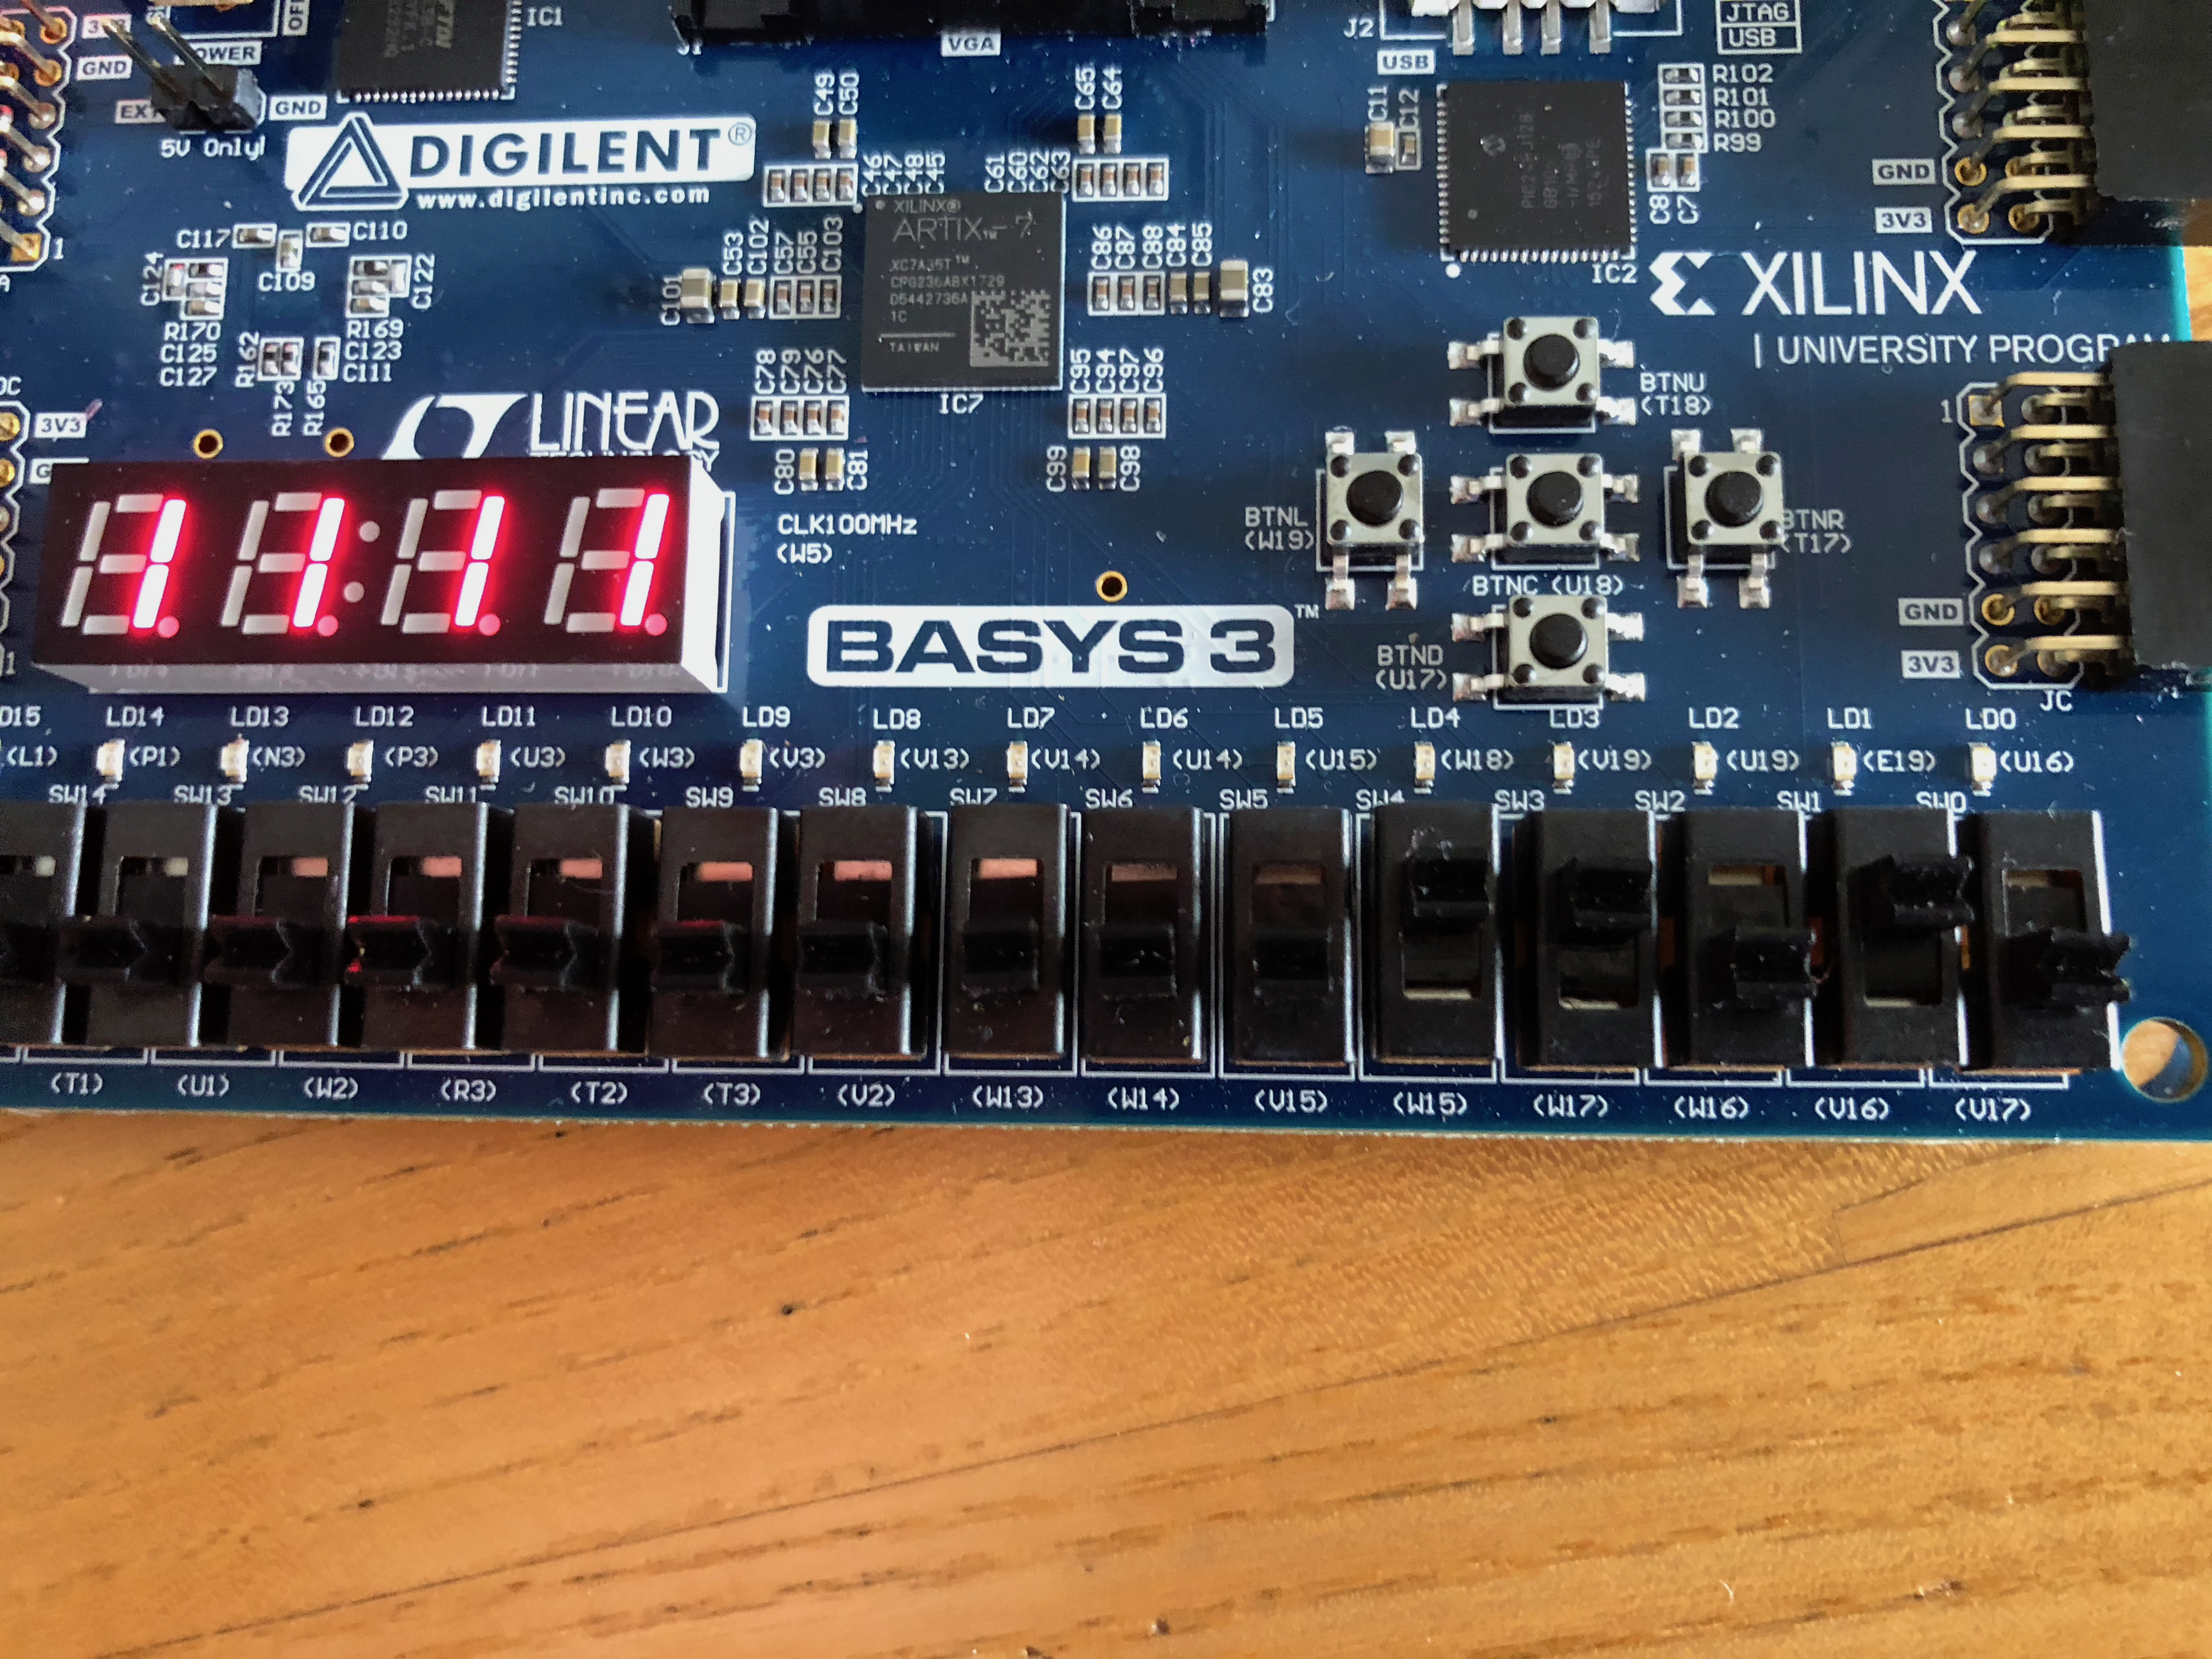
\includegraphics[width=0.4\textwidth]{./report-images/Part3/IMG_0477.png}
	\caption{\label{fig:sevSegOnePlusTwoPlusTwoCarry}In this image, carry-in is 1, B is 10, and A is 10. The decimal equivalent is 1 + 2 + 2 = 5. Because the select switch is off, the output is the carry out of the equation which is one.}
\end{center}
\end{figure}

\begin{figure}[H]
\begin{center}
	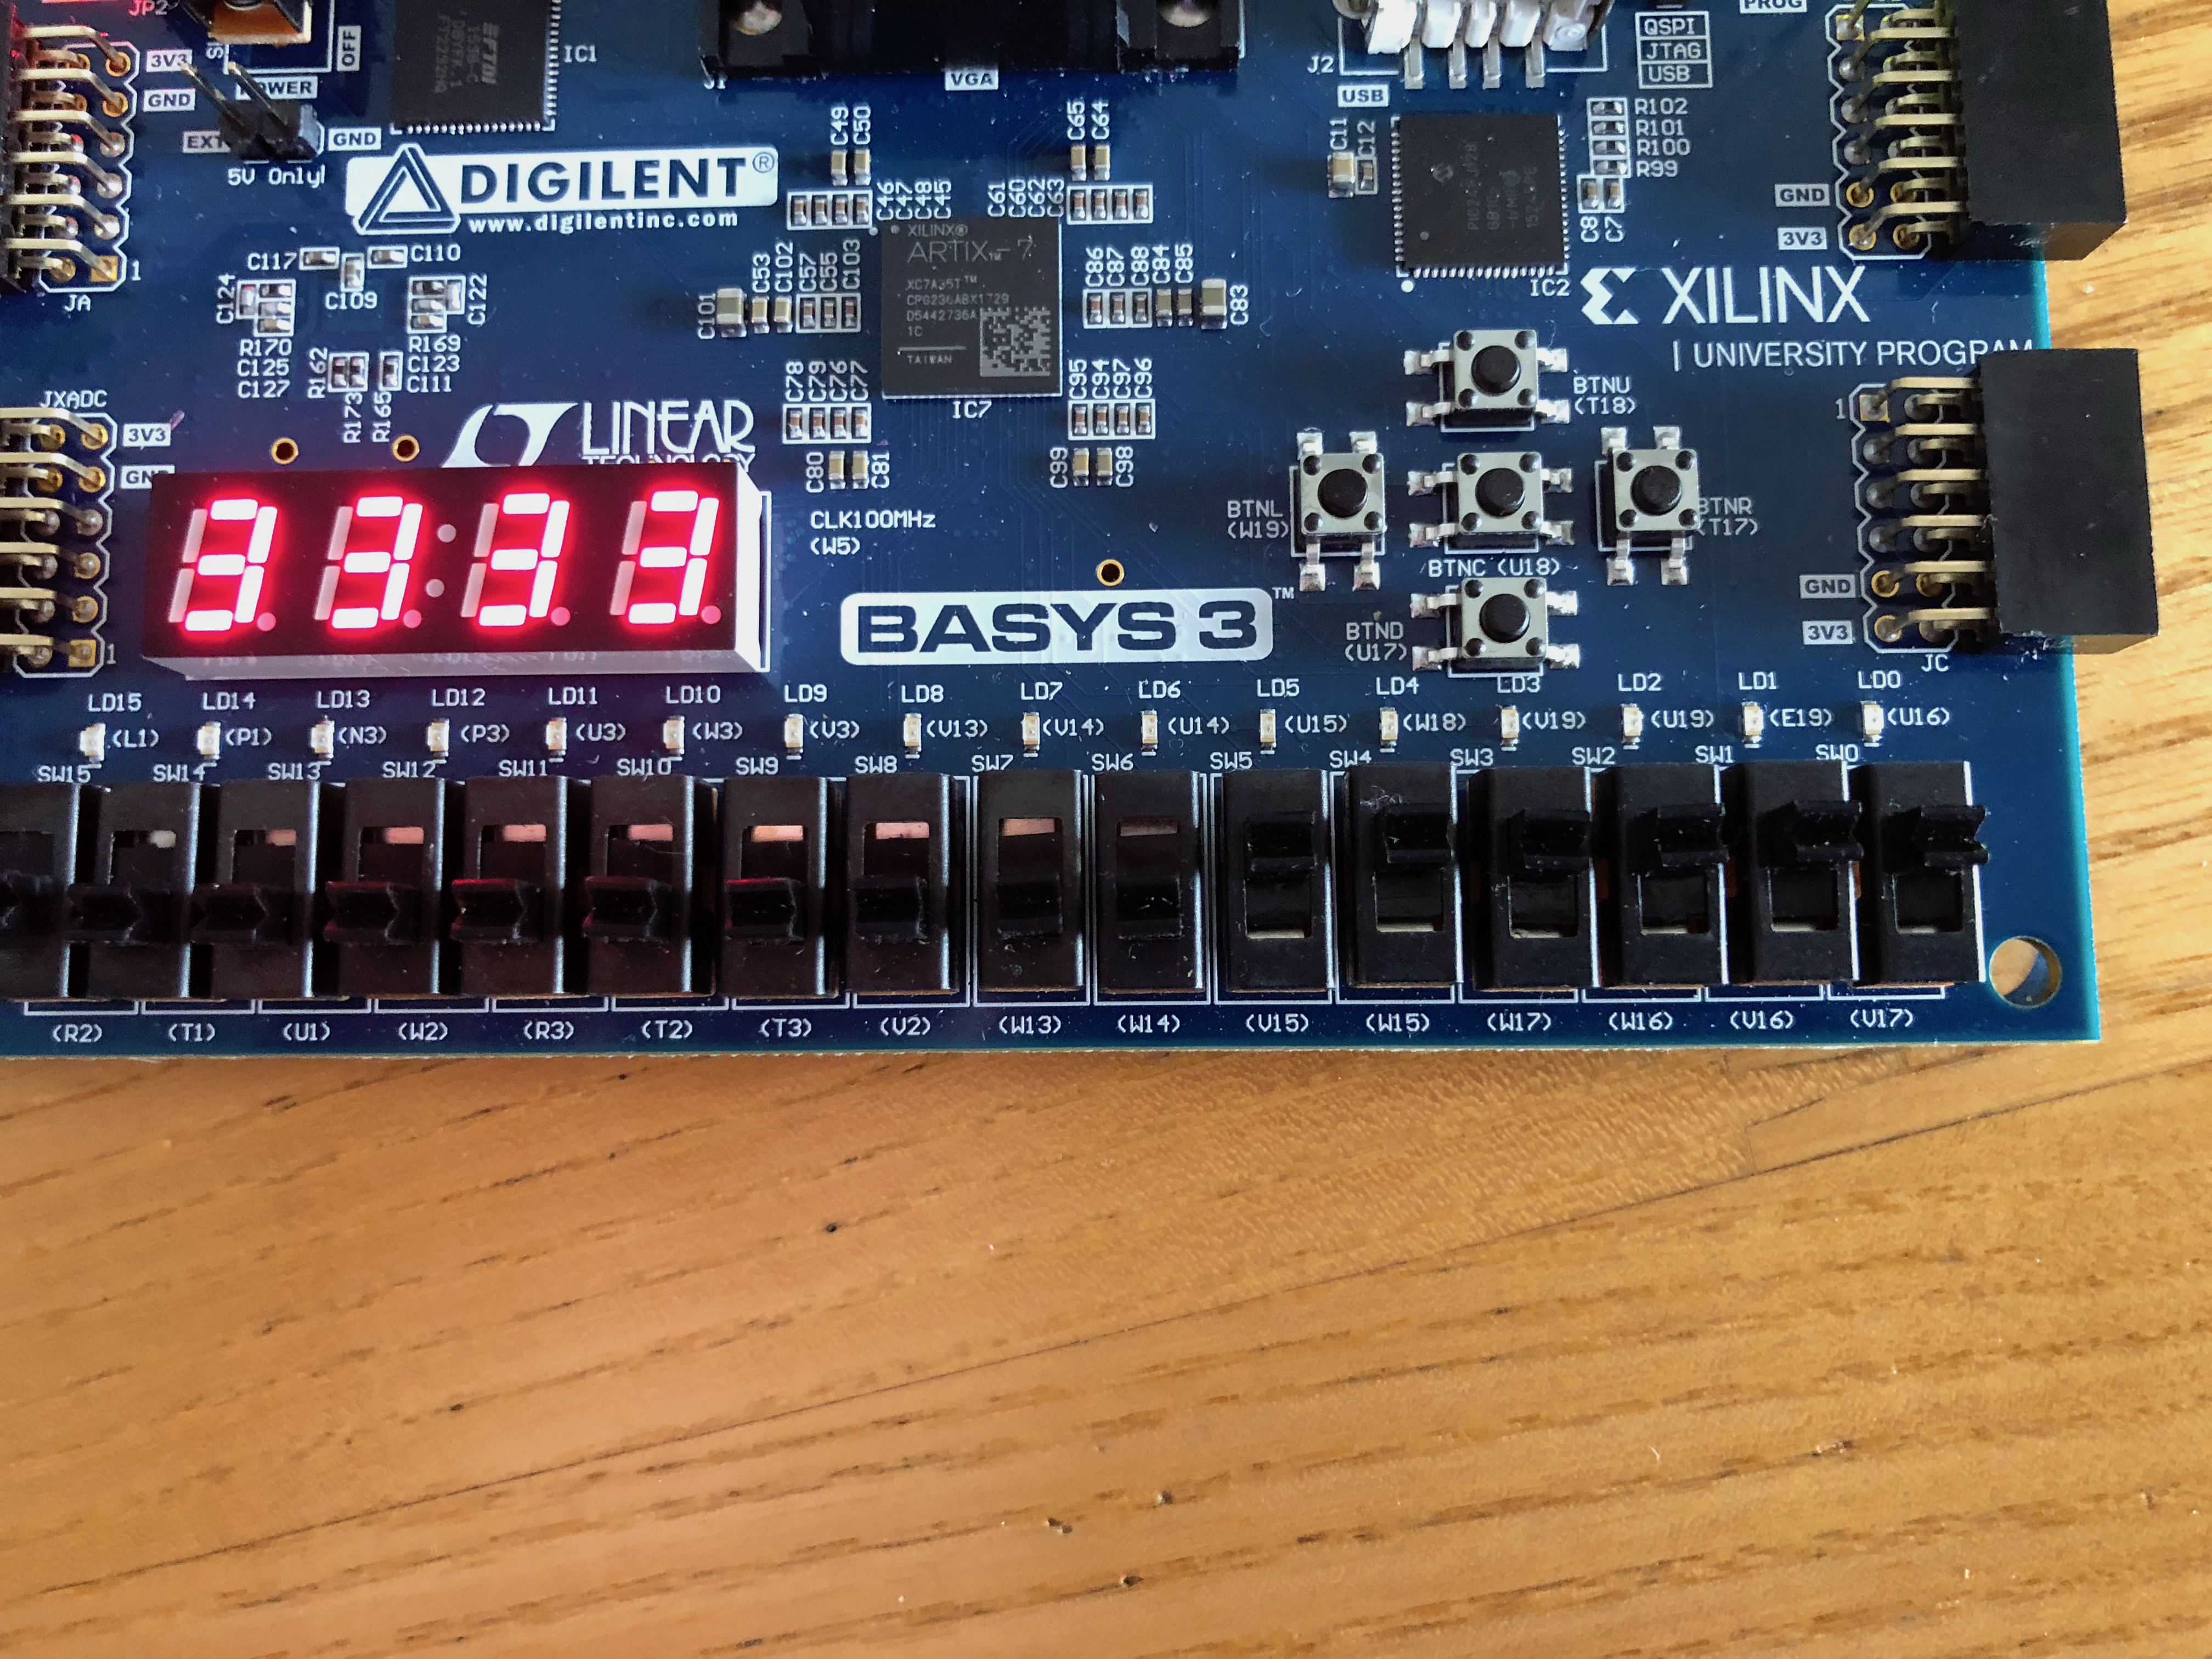
\includegraphics[width=0.4\textwidth]{./report-images/Part3/IMG_0478.png}
	\caption{\label{fig:sevSegOnePlusThreePlusThreeSUM}In this image, carry-in is 1, B is 11, and A is 11. The decimal equivalent is 1 + 3 + 3 = 7. Because the select switch is on, the output is the sum of the equation which is 3. The other 4 would be stored in the carry out.}
\end{center}
\end{figure}

\begin{figure}[H]
\begin{center}
	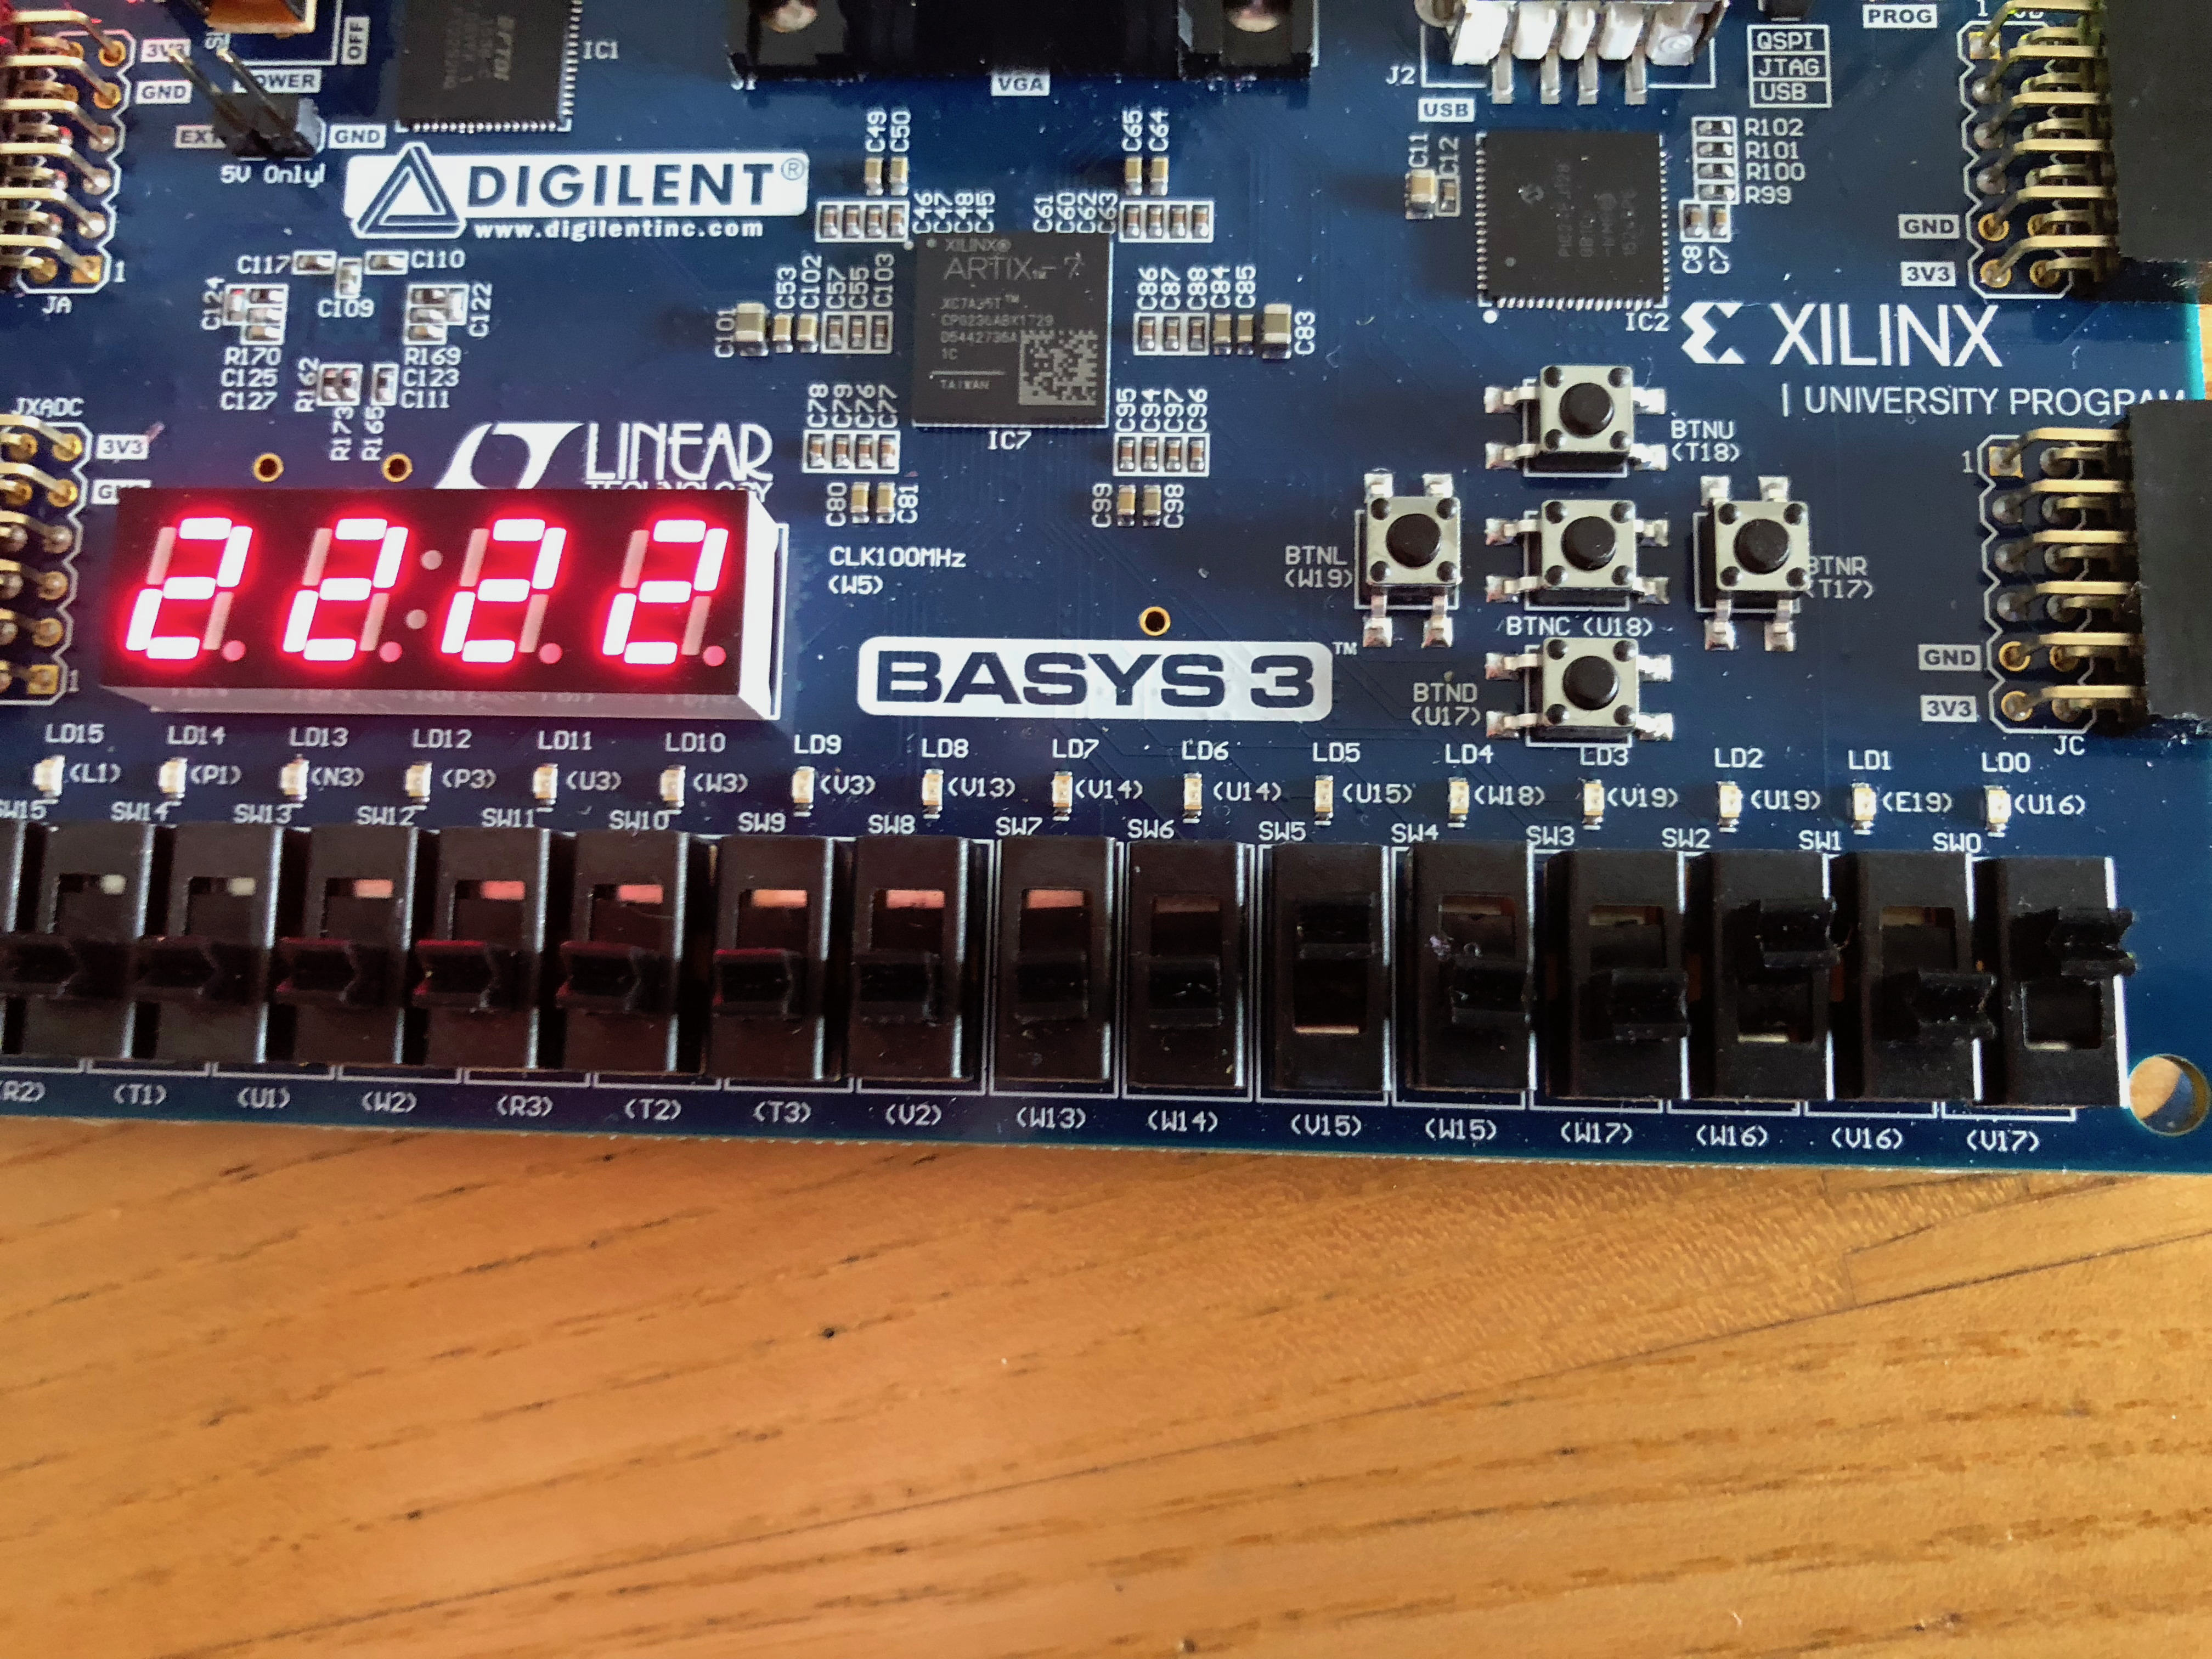
\includegraphics[width=0.4\textwidth]{./report-images/Part3/IMG_0479.png}
	\caption{\label{fig:sevSegOnePlusOneSUM}In this image, carry-in is 0, B is 01, and A is 01. The decimal equivalent is 0 + 1 + 1 = 2. Because the select switch is on, the output is the sum of the equation which is two and can be displayed in the seven-segment display.}
\end{center}
\end{figure}

\section{Conclusion}
This lab taught us many new things about using components to build a complex system. The most technically challenging part of this lab was the multiple syntax errors possible in such a large system, with many different entities working together. After completing this lab, we are confident in our ability to work with VHDL components to create complex systems.

\pagebreak

\textbf{Appendices}

\begin{appendices}

\section{Problem 1 VHDL Code}

\begin{lstlisting}[language=VHDL]
library IEEE;
use IEEE.STD_LOGIC_1164.ALL;

-- This entity represents a single bit full adder. It will add a and b along 
-- with cin, and provide output in sum and cout.
entity full_adder is

    Port ( cin : in STD_LOGIC;

           a : in STD_LOGIC;

           b : in STD_LOGIC;

           cout : out STD_LOGIC;

           sum : out STD_LOGIC);

end full_adder;

architecture Behavioral of full_adder is
begin

-- The architecture for the full adder handles simple logic to determine 
-- sum and cout independently

sum <= (a and b and cin) or (a and (not b) and (not cin)) or (b and (not a) 
	and (not cin)) or (cin and (not a) and (not b));
cout <= (cin and (a or b)) or (a and b);
end Behavioral;

library IEEE;
use IEEE.STD_LOGIC_1164.ALL;

-- The two-bit adder will utilize two of the full adders defined above
-- to add respective bits separately
entity two_bit_adder is
    Port ( cin : in STD_LOGIC;
           a2 : in STD_LOGIC;
           a1 : in STD_LOGIC;
           b2 : in STD_LOGIC;
           b1 : in STD_LOGIC;
           x2 : out STD_LOGIC;
           x1 : out STD_LOGIC;
           cout : out STD_LOGIC);
end two_bit_adder;

architecture Behavioral_Two of two_bit_adder is

-- This component will utilize the logic defined in the full adder above
component full_adder port (a, b, cin : in STD_LOGIC; sum, cout : out STD_LOGIC);
end component full_adder;

-- This signal will carry the carry-out from the least significant addition to the 
-- carry-in of the most significant addition
signal c1 : STD_LOGIC;

begin
-- Uses two instances of the full adder component to complete the calculation
    adder_one : full_adder port map(a1, b1, cin, x1, c1);
    adder_two : full_adder port map(a2, b2, c1, x2, cout);

end Behavioral_Two;

\end{lstlisting}

\section{Problem 1 Constraints File}
\begin{figure}[H]
\begin{center}
	\includegraphics[width=0.5\textwidth]{./report-images/Part2/P2Const.png}
	\caption{\label{fig:Part1ConstFile}Constraints file for Problem 1.}
\end{center}
\end{figure}

\section{Problem 2 VHDL Code}
\begin{lstlisting}[language=VHDL]
library IEEE;
use IEEE.STD_LOGIC_1164.ALL;

-- This entity represents a single bit full adder. It will add a and b along with 
-- cin, and provide output in sum and cout.
entity full_adder is

    Port ( cin : in STD_LOGIC;

           a : in STD_LOGIC;

           b : in STD_LOGIC;

           cout : out STD_LOGIC;

           sum : out STD_LOGIC);

end full_adder;

architecture Behavioral of full_adder is
begin

-- The architecture for the full adder handles simple logic to determine sum 
-- and cout independently

sum <= (a and b and cin) or (a and (not b) and (not cin)) or (b and (not a) and 
	(not cin)) or (cin and (not a) and (not b));
cout <= (cin and (a or b)) or (a and b);
end Behavioral;

library IEEE;
use IEEE.STD_LOGIC_1164.ALL;

-- The two-bit adder will utilize two of the full adders defined above to 
-- add respective bits separately
entity two_bit_adder is
    Port ( cin : in STD_LOGIC;
           a2 : in STD_LOGIC;
           a1 : in STD_LOGIC;
           b2 : in STD_LOGIC;
           b1 : in STD_LOGIC;
           x2 : out STD_LOGIC;
           x1 : out STD_LOGIC;
           cout : out STD_LOGIC);
end two_bit_adder;

architecture Behavioral_Two of two_bit_adder is

-- This component will utilize the logic defined in the full adder above
component full_adder port (a, b, cin : in STD_LOGIC; sum, cout : out STD_LOGIC);
end component full_adder;

-- This signal will carry the carry-out from the least significant addition
-- to the carry-in of the most significant addition
signal c1 : STD_LOGIC;

begin
-- Uses two instances of the full adder component to complete the calculation
    adder_one : full_adder port map(a1, b1, cin, x1, c1);
    adder_two : full_adder port map(a2, b2, c1, x2, cout);

end Behavioral_Two;

library IEEE;
use IEEE.STD_LOGIC_1164.ALL;

entity Lab3Part2 is
    Port ( cin : in STD_LOGIC;
           a1 : in STD_LOGIC;
           a2 : in STD_LOGIC;
           b1 : in STD_LOGIC;
           b2 : in STD_LOGIC;
           sel : in STD_LOGIC;
           x2 : out STD_LOGIC;
           x1: out STD_LOGIC);
end Lab3Part2;

architecture Behavioral_Three of Lab3Part2 is
component two_bit_adder port(cin, a2, a1, b2, b1 : in STD_LOGIC; x2, x1, 
	cout : out STD_LOGIC);
end component two_bit_adder;
signal sum1 : STD_LOGIC;
signal sum2 : STD_LOGIC;
signal tmpc : STD_LOGIC;

begin
    adder : two_bit_adder port map(cin, a2, a1, b2, b1, sum2, sum1, tmpc);
    
    x2 <= '0' when (sel_a = '0') else sum2;
    x1 <= tmpc when (sel_a = '0') else sum1;    

end Behavioral_Three;
\end{lstlisting}

\section{Problem 2 Constraints File}
\begin{figure}[H]
\begin{center}
	\includegraphics[width=0.5\textwidth]{./report-images/Part2/P2Const.png}
	\caption{\label{fig:Part2ConstFile}Constraints file for Problem 2.}
\end{center}
\end{figure}

\section{Problem 3 VHDL Code}
\begin{lstlisting}[language=VHDL]
library IEEE;
use IEEE.STD_LOGIC_1164.ALL;

-- This entity represents a single bit full adder. It will add a and b along with 
-- cin, and provide output in sum and cout.
entity full_adder is

    Port ( cin : in STD_LOGIC;

           a : in STD_LOGIC;

           b : in STD_LOGIC;

           cout : out STD_LOGIC;

           sum : out STD_LOGIC);

end full_adder;

architecture Behavioral of full_adder is
begin

-- The architecture for the full adder handles simple logic to determine sum 
-- and cout independently

sum <= (a and b and cin) or (a and (not b) and (not cin)) or (b and (not a) and 
	(not cin)) or (cin and (not a) and (not b));
cout <= (cin and (a or b)) or (a and b);
end Behavioral;

library IEEE;
use IEEE.STD_LOGIC_1164.ALL;

-- The two-bit adder will utilize two of the full adders defined above to 
-- add respective bits separately
entity two_bit_adder is
    Port ( cin : in STD_LOGIC;
           a2 : in STD_LOGIC;
           a1 : in STD_LOGIC;
           b2 : in STD_LOGIC;
           b1 : in STD_LOGIC;
           x2 : out STD_LOGIC;
           x1 : out STD_LOGIC;
           cout : out STD_LOGIC);
end two_bit_adder;

architecture Behavioral_Two of two_bit_adder is

-- This component will utilize the logic defined in the full adder above
component full_adder port (a, b, cin : in STD_LOGIC; sum, cout : out STD_LOGIC);
end component full_adder;

-- This signal will carry the carry-out from the least significant addition
-- to the carry-in of the most significant addition
signal c1 : STD_LOGIC;

begin
-- Uses two instances of the full adder component to complete the calculation
    adder_one : full_adder port map(a1, b1, cin, x1, c1);
    adder_two : full_adder port map(a2, b2, c1, x2, cout);

end Behavioral_Two;

library IEEE;
use IEEE.STD_LOGIC_1164.ALL;

-- The mux adder has one less input because it will only display up to 2 bits
--  at a time.
-- The inputs are the same as a 2-bit slicer with a select bit
entity mux_adder is
    Port ( cin : in STD_LOGIC;
           y1 : in STD_LOGIC;
           y2 : in STD_LOGIC;
           z1 : in STD_LOGIC;
           z2 : in STD_LOGIC;
           sel_a : in STD_LOGIC;
           x2 : out STD_LOGIC;
           x1: out STD_LOGIC);
end mux_adder;

-- The architecture will display the sum when sul is high and the cout when
-- select is low
architecture Behavioral_Three of mux_adder is
component two_bit_adder port(cin, y2, y1, z2, z1 : in STD_LOGIC; x2, x1, 
	cout : out STD_LOGIC);
end component two_bit_adder;
signal sum1 : STD_LOGIC;
signal sum2 : STD_LOGIC;
signal tmpc : STD_LOGIC;

begin
-- This instantiates an instance of the two bit slicer defined above and 
-- detailed in Problem 2
    adder : two_bit_adder port map(cin, y2, y1, z2, z1, sum2, sum1, tmpc);
    process(sel)
        being
        x2 <= '0' when (sel_a = '0') else sum2;
        x1 <= tmpc when (sel_a = '0') else sum1;
    end process;
    

end Behavioral_Three;

library IEEE;
use IEEE.STD_LOGIC_1164.ALL;

-- This entity takes in the information for a 2:1 mux and outputs it to 7-segment
-- Displays
entity Lab3Part3 is
    Port ( a2 : in STD_LOGIC;
           a1 : in STD_LOGIC;
           b2 : in STD_LOGIC;
           b1 : in STD_LOGIC;
           cin : in STD_LOGIC;
           sel : in STD_LOGIC;
           out1 : out STD_LOGIC;
           out2 : out STD_LOGIC;
           out3 : out STD_LOGIC;
           out4 : out STD_LOGIC;
           out5 : out STD_LOGIC;
           out6 : out STD_LOGIC;
           out7 : out STD_LOGIC);
end Lab3Part3;

architecture Behavioral of Lab3Part3 is
component mux_adder port(cin, y1, y2, z1, z2, sel : in STD_LOGIC; 
	x2, x1 : out STD_LOGIC);
end component mux_adder;

signal c_sig : bit;
signal x1_sig : bit;
signal x2_sig : bit;

begin

adder : mux_adder port map(cin => cin, y1 => a1, y2 => a2, z1 => b1, z2 => b2, 
	sel_a => sel, x2 => x2_sig, x1 => x1_sig, cout => c_sig);

process (sel)
--when sel is  high then display shows 3,2,1,0 depend on x2 and x1 when sel 
-- is low then display shows 0, or 1 depend on cout
   begin
   case sel is 
   when '0' =>
    if cout = '0' then
      out1 <= '0';
      out2 <= '0';
      out3 <= '0';
      out4 <= '0';
      out5 <= '0';
      out6 <= '0';
      out7 <= '1';
   else
    out1 <= '1';
    out2 <= '0';
    out3 <= '0';
    out4 <= '1';
    out5 <= '1';
    out6 <= '1';
    out7 <= '1';
    end if;
   
                 
 when '1' =>   
 if (x2='0'and x1='0')then
                out1 <= '0';
                out2 <= '0';
                out3 <= '0';
                out4 <= '0';
                out5 <= '0';
                out6 <= '0';
                out7 <= '1';  
 elsif (x2='0'and x1='1')then
                 out1 <= '1';
                 out2 <= '0';
                 out3 <= '0';
                 out4 <= '1';
                 out5 <= '1';
                 out6 <= '1';
                 out7 <= '1'; 
 elsif (x2='1'and x1='0')then           
                 out1 <= '0';
                 out2 <= '0';
                 out3 <= '1';
                 out4 <= '0';
                 out5 <= '0';
                 out6 <= '1';
                 out7 <= '0'; 
                                 
   elsif (x2='1'and x1='1')then   
                 out1 <= '0';
                 out2 <= '0';
                 out3 <= '0';
                 out4 <= '0';
                 out5 <= '1';
                 out6 <= '1';
                 out7 <= '0';  
                 
   end if;                                   
                             
   end case;
   end process;              
end Behavioral;

\end{lstlisting}

\section{Problem 3 Constraints File}
\begin{figure}[H]
\begin{center}
	\includegraphics[width=0.5\textwidth]{./report-images/Part3/P3Const.png}
	\caption{\label{fig:Part3ConstFile}Constraints file for Problem 3.}
\end{center}
\end{figure}
\end{appendices}
\end{document}
